\documentclass[runningheads]{llncs}
%
\usepackage[T1]{fontenc}
% T1 fonts will be used to generate the final print and online PDFs,
% so please use T1 fonts in your manuscript whenever possible.
% Other font encondings may result in incorrect characters.
%
\usepackage{amsmath}
\usepackage{graphicx}
\usepackage{nameref}
\usepackage{varioref}
\usepackage{hyperref}
\usepackage{cleveref}
\usepackage{multirow}
\usepackage{svg}

\usepackage{longtable}
\usepackage{hhline}
% Used for displaying a sample figure. If possible, figure files should
% be included in EPS format.
%
% If you use the hyperref package, please uncomment the following two lines
% to display URLs in blue roman font according to Springer's eBook style:
\usepackage{color, colortbl}
%\renewcommand\UrlFont{\color{blue}\rmfamily}
%
\usepackage{tikz}
\usepackage{tikzit}
\input{sample.tikzstyles}
\def\chm{\tikz\fill[scale=0.4](0,.35) -- (.25,0) -- (1,.7) -- (.25,.15) -- cycle;}
\def\crs{\tikz[scale=0.25, line width=0.3mm]\draw(0,0) -- (1,1) (0,1) -- (1,0);}

\def\pbox{\parbox{6cm}}

\begin{document}
\title{
    SemEval 2024 Task 2: Safe Biomedical Natural Language Inference for Clinical Trials
    %\thanks{Supported by organization x.}
}
%
%\titlerunning{Abbreviated paper title}
% If the paper title is too long for the running head, you can set
% an abbreviated paper title here
%
\author{Raphael Baumann\inst{1}\orcidID{2909063}}
%
\authorrunning{R. Baumann}
% First names are abbreviated in the running head.
% If there are more than two authors, 'et al.' is used.
%
\institute{
Chair of Natural Language Processing \\ 
Institute of Computer Science \\
Faculty of Mathematics and Computer Science \\ 
Julius-Maximilians University of Würzburg \\ 
Würzburg, Germany\\
\email{raphael.baumann@stud-mail.uni-wuerzburg.de} \\
}




\maketitle              % typeset the header of the contribution

\begingroup %\input{} or %\include{}
\begin{abstract}
	TODO
	\keywords{Natural Language Processing (NLP)\and
		Large Language Models (LLMs)  \and
		BERT \and
		Transformer \and
		Machine Learning \and
		Artificial  Intelligence}
\end{abstract}
%\newpage
\section{Introduction}\label{sec:introduction}



In clinical studies, Clinical Trial Reports (CTRs) provide detailed information about patients
treatments and reactions \cite{noauthor_nli4ct_nodate} \cite{jullien_nli4ct_2023}. 
However, the increasing volume of CTRs, coupled with a lack of suitable 
analytical tools, poses challenges for clinicians to deliver personalized, evidence-based care \cite{takehana_stanford_2023}\cite{wang_knowcomp_2023}. 
Despite improvements in CTR reliability, there is a notable gap in the ability to analyze and compare them effectively \cite{vladika_sebis_2023}. 
Natural language inference (NLI) models show promise in deducing logical relationships in texts, but their application 
in the medical domain presents unique challenges \cite{wang_knowcomp_2023}\cite{alissa_just-km_2023}\cite{rajamanickam_i2r_2023}\cite{takehana_stanford_2023}\cite{vladika_sebis_2023}. 
These include the need for domain-specific knowledge due to clinical 
jargon and the variability in scientific communication. Additionally, distinguishing between non-entailed subsequences 
further complicates NLI systems \cite{noauthor_nli4ct_nodate}.


\paragraph{\textbf{Task:}} Classification of the relation between CTR premises and a 
statement, as being Entailed or a Contradiction. Models are expected to predict whether 
each statement affirms an entailment or forms a contradiction given the associated 
section from the claimed CTRs.


Recent works are reviewed, highlighting shortcomings in existing systems. 
Various models are examined, employing strategies such as pipeline concatenation, 
joint representation, supervised contrastive learning, and role-based enhancement \cite{wang_knowcomp_2023}\cite{alissa_just-km_2023}\cite{vladika_sebis_2023}\cite{zhou_thifly_2023}.
We are clarifying in Chapter~\ref{sec:dataset} how the CTR Dataset for the SemEval Task 2
is built and how we use them in our Models and Strategies. Also, we are briefly looking into the 
ranking of several, mostly BERT derivatives, Models.
Methods, detailed in the Chapter~\ref{sec:methods}, cover loss and metric functions, 
the use of BERT as the base model, sentence embedding architectures 
like SBERT, and adapter tuning. Experiments in constrained environments 
explore learning rate effects, token size challenges, and the impact of sentence 
permutation. Dataset expansion strategies and the effects of different sentence 
embedding architectures and adapter tuning on model performance are thoroughly evaluated.
The experiments (see Chapter~\ref{sec:experiments}) collectively shed light on the complexities of clinical trial report analysis, 
emphasizing the need to address challenges in data processing, model architecture, and training 
strategies.








\newpage
\section{Datasets}\label{sec:dataset}

\begin{table}[!b]
    \centering
    \caption{Two Example Clinical Trial Report taken out of the Dataset to represent the two types Comparison and Single.
             Each Sample has a Statement, Label, the relevant Section and one or two Premises called Trial.}
    \label{tab:ds-example}
    \resizebox{\textwidth}{!}{%
    \begin{tabular}{|l||c|l|l|}
    \hline
    Type            & Short                                                         & Comparison                                                                                                                                                                                                                                                                                                                                                                            & Single                                                                                                                                                                                                                                                                                                                                                         \\ \hline\hline
    Label           &                                                               & Entailment                                                                                                                                                                                                                                                                                                                                                                            & Contradiction                                                                                                                                                                                                                                                                                                                                                  \\ \hline
    \textcolor{red}{Statement}       & \textcolor{red}{stm}                                                           & \textcolor{red}{\begin{tabular}[c]{@{}l@{}}The primary trial and the secondary \\ trial both used MRI for their interventions.\end{tabular}}                                                                                                                                                                                                                                                           & \textcolor{red}{\begin{tabular}[c]{@{}l@{}}More than 1/3 of patients in cohort 1 of the\\ primary trial experienced an adverse event.\end{tabular}}                                                                                                                                                                                                                             \\ \hline
    \textcolor{green}{Section}         & \textcolor{green}{sec}                                                           & \textcolor{green}{Intervention}                                                                                                                                                                                                                                                                                                                                                                          & \textcolor{green}{Adverse Events}                                                                                                                                                                                                                                                                                                                                                 \\ \hline
    \textcolor{blue}{Primary Trial}   & \textcolor{blue}{\begin{tabular}[c]{@{}l@{}}$p_1$\\ $p_2$\\ $...$\end{tabular}} & \textcolor{blue}{\begin{tabular}[c]{@{}l@{}}INTERVENTION 1:\\ •  Letrozole, Breast Enhancement, Safety\\ • Single arm of healthy postmenopausal women to \\    have two breast MRI (baseline and post-treatment). \\    Letrozole of 12.5 mg/day is given for three successive \\    days just prior to the second MRI.\\ • ...\end{tabular}}                                                           & \textcolor{blue}{\begin{tabular}[c]{@{}l@{}}Adverse Events 1:\\ •  Total: 69/258 (26.74\%)\\ •  Anaemia 3/258 (1.16\%)\\ •  Febrile neutropenia 13/258 (5.04\%)\\  •  Neutropenia 5/258 (1.94\%)\\  • ...\\ Adverse Events 2:\\ •  Mitral valve incompetence 0/224 (0.00\%)\\ •  Pericardial effusion 2/224 (0.89\%)\\ •  Sinus tachycardia 1/224 (0.45\%)\\ • ...\end{tabular}} \\ \hline
    \textcolor{blue}{Secondary Trial} & \textcolor{blue}{\begin{tabular}[c]{@{}l@{}}$s_1$\\ $s_2$\\ $...$\end{tabular}} & \textcolor{blue}{\begin{tabular}[c]{@{}l@{}}INTERVENTION 1: \\ •  Healthy Volunteers\\ • Healthy women will be screened for \\    Magnetic Resonance Imaging (MRI)  contraindications, \\    and then undergo contrast injection, and SWIFT acquisition.\\ •  Magnetic resonance imaging: Patients and healthy volunteers \\    will be first screened for MRI contraindications.\\ • ...\end{tabular}} &                                                                                                                                                                                                                                                                                                                                                                \\ \hline
    \end{tabular}%
    }
\end{table}

A group of four domain experts, including clinical trial organizers from the Manchester Cancer Institute and the 
Digital Experimental Cancer Medicine Team (DECMT), participated in an annotation task to generate entailment and contradiction 
statements for Clinical Trial Reports (CTR). Annotators were tasked with generating non-trivial statements about the contents of primary and 
secondary trials, encouraging understanding and reasoning. Each CTR was divided into four sections representing facts, and 
evidence supporting the labeled statement was selected from these facts. In cases of negation, the full CTR section was 
provided as evidence. A negative rewriting strategy was employed to create contradictory statements, and evidence contradicting 
these statements was collected \cite{jullien_semeval-2023_nodate} \cite{noauthor_nli4ct_nodate}.
Each Datapoint in the Training and Development Set have a statement, label being either Entangled or Contradiction, and one or two Prompts being
one of four different CTR sections of Adverse Events, Eligibility, Intervention or Results (see Table~\ref{tab:ds-example}). 
60\% of the Dataset are Single-Type, which then has only the Primary Prompt as relevant information and the other 40\% are 
Comparison-Type has Primary and Secondary Prompt \cite{noauthor_nli4ct_nodate}\cite{jullien_nli4ct_2023}\cite{jullien_semeval-2023_nodate}.
The SemEval task 2 dataset consists of 1700 training and 200 development samples (see Table~\ref{tab:ds-distribution}),
distributed equally between the two labels and almost for the 4 kinds of CTR sections. We use the development samples
as validation dataset to evaluate the performance of the Models.


\begin{table}[t]
    \centering
    \caption{Section and Label Distribution of the Training and Validation Dataset, showing
             an almost equal distribution torough the four Sections.}
    \label{tab:ds-distribution}
    \begin{tabular}{|c|c||cccc|c|c|}
    \hline
    \multirow{2}{*}{Dataset} & \multirow{2}{*}{Label} & \multicolumn{4}{c|}{Section} & \multirow{2}{*}{$\Sigma$} & \multirow{2}{*}{Total} \\
                           &               & Adverse Events & Eligibility & Intervention & Results &     &                       \\ \hline\hline
    \multirow{2}{*}{train} & Contradiction & 238            & 241         & 196          & 175     & 850 & \multirow{2}{*}{1700} \\
                           & Entailment    & 258            & 245         & 200          & 147     & 850 &                       \\ \hline
    \multirow{2}{*}{valid} & Contradiction & 26             & 28          & 18           & 28      & 100 & \multirow{2}{*}{200}  \\
                           & Entailment    & 26             & 28          & 18           & 28      & 100 &                       \\ \hline
    \end{tabular}
\end{table}


\begin{figure}[!b]
    \centering
    \includesvg[inkscapelatex=false, width=\textwidth]{./content/histogram}
    \caption{Histogram of Number of Words from the full Sentence and the tokenized version with BertTokenizer, 
             with 70\% are in line of 512 Tokens for both.}\label{cap:hist}
\end{figure}

For our further proceeding we concatenate the parts of a dataset sample as followed in Equation~\ref{eq:ds-sentence}.
The Single-Type, where there is no Second Trial (see Table~\ref{tab:ds-example}), $s_1, s_2, ... $
is empty, so the two last $[SEP]$ tokens are directly after another and for Comparison Type are all elements given, 
therefore the Sentence is exactly:

\begin{equation}\label{eq:ds-sentence}
\resizebox{0.91\hsize}{!}{%
 $Sentence = [CLS] \; \textcolor{red}{stm}\;
             [SEP] \; \textcolor{green}{sec}\;
             [SEP] \; \textcolor{blue}{p_1, p_2, ... }\;
             [SEP] \; \textcolor{blue}{s_1, s_2, ... }\;
             [SEP]$      
}
\end{equation}

As our base Model for our Experiments is BERT and the respective Tokenizer uses $512$ token, to encode the Sentence, 
we have analyzed the length Distribution in a Histogram (see Figure~\ref{cap:hist}). 
Round about 70\% of all Training and Validation Datapoints are in the range of the $512$ token length. 
Visible is also the slight shift on the $x$-Axis in the tokenized form, since not every word can have a single token
representing it.
\section{Recent Works}\label{sec:recentworks}


The majority of the released systems failed to achieve significantly above the majority-class baseline of 66.7\%
F1 value see Table~\ref{tab:results} \cite{jullien_semeval-2023_nodate}.
\textbf{Sebis \cite{vladika_sebis_2023}} uses a system concatenating the parts of the CTRs in two diffent method, called pipeline and joint, 
where basically the sentence represenation includes more $[SEP]$ tokens to dense it up.
\textbf{KnowComp \cite{wang_knowcomp_2023}, YNU-HPCC \cite{feng_ynu-hpcc_nodate} and Stanford \cite{takehana_stanford_2023}, I2R \cite{rajamanickam_i2r_2023}, Clemson NLP \cite{alameldin_clemson_nodate}} uses the same strategy as we do (see Equation ~\ref{eq:ds-sentence}) to feed forward the sentence in several most popular Models.
Compared to the others, \textbf{YNU-HPCC \cite{feng_ynu-hpcc_nodate}} utilize Supervised Contrastive Learning with the corresponding loss function.
\textbf{JUST-KM \cite{alissa_just-km_2023}} Models are enhanching RoBERTa in a role-based approach, where the two RoBERTa-Large Models trained differently, 
to predict the general outcome.
\textbf{Saama \cite{kanakarajan_saama_2023}} finetuned Flan-T5 LLM to SemEval's task-specific data by applying different Instruction Templates. 
\textbf{THiFLY \cite{zhou_thifly_2023}} employ Multigranularity Inference Network, which uses the Equation~\ref{eq:ds-sentence} sentence structure to pass
it further to a Joint Semantic Encoder followed by Pooling and Sencence-Level Encoder before Classification.




\begin{table}[]
    \centering
    \caption{Results of the SemEval-2023 Task 7.1 (SemEval-2024 Task 2) \cite{noauthor_nli4ct_nodate}, with
             several attempts to use BERT as baseline.}
    \label{tab:results}
    \begin{tabular}{|l||l|l|}
    \hline
    Model/Method     & Working Team                                                             & F1                                                                                       \\ \hline\hline
    BERT             & \begin{tabular}[c]{@{}l@{}}KnowComp\\ Sebis\\ JUST-KM\end{tabular}   & \begin{tabular}[c]{@{}l@{}}base: 69.2 large: 70.9\\ base: 61:0\\ base: 63.4\end{tabular} \\ \hline
    DistilBERT       & Standford                                                            & 60.8                                                                                     \\ \hline
    BioBERT          & \begin{tabular}[c]{@{}l@{}}Sebis\\ Standford\\ YNU-HPCC\end{tabular} & \begin{tabular}[c]{@{}l@{}}64.5\\ 63.7\\ 67.9\end{tabular}                               \\ \hline
    BioClinical-BERT & \begin{tabular}[c]{@{}l@{}}KnowComp\\ Sebis\\ Standford\end{tabular} & \begin{tabular}[c]{@{}l@{}}65.3\\ 65.7\\ 64.8\end{tabular}                               \\ \hline
    GatorTron-BERT   & Clemson NLP                                                          & 70.5                                                                                     \\ \hline
    PubMedBERT       & Standford                                                            & 66.0                                                                                     \\ \hline
    ALBERT-v2        & KnowComp                                                             & 67.1                                                                                     \\ \hline
    BART             & KnowComp                                                             & base: 67.1 large: 66.9                                                                   \\ \hline
    RoBERTa          & \begin{tabular}[c]{@{}l@{}}KnowComp\\ JUST-KM\end{tabular}           & \begin{tabular}[c]{@{}l@{}}base: 70.7 large: 67.6\\ base: 65.6 large: 66.1 role-based: 67.0\end{tabular}  \\ \hline
    DeBERTa-v3       & \begin{tabular}[c]{@{}l@{}}KnowComp\\ Sebis\end{tabular}             & \begin{tabular}[c]{@{}l@{}}base: 75.8 large: 81.5\\ large: 80.5\end{tabular}             \\ \hline
    ELECTRA          & \begin{tabular}[c]{@{}l@{}}KnowComp\\ Standford\end{tabular}         & \begin{tabular}[c]{@{}l@{}}base:70.3 large: 76.1\\ small: 63.9\end{tabular}              \\ \hline
    GPT2             & KnowComp                                                             & base: 39.0 medium 44.2 large: 61.5                                                       \\ \hline
    T5               & I2R                                                                  & base: 62.9 large: 68.3                                                                   \\ \hline
    Flan-T5-xxl      & Saama                                                                & 83.4                                                                                     \\ \hline
    MGNet            & THiFLY                                                               & 85.6                                                                                     \\ \hline
    \end{tabular}
\end{table}

\newpage
\section{Methods}\label{sec:methods}
In this chapter we are clarifying the Loss and Metric Functions, the Architecture BERT used for our Experiments, Ideas principles like Adapter Tuning and
Sentence Embedding and how fusing different Dataset together works, which are used in training loop.


\subsection{BERT}
\begin{figure}[b]
    \centering
    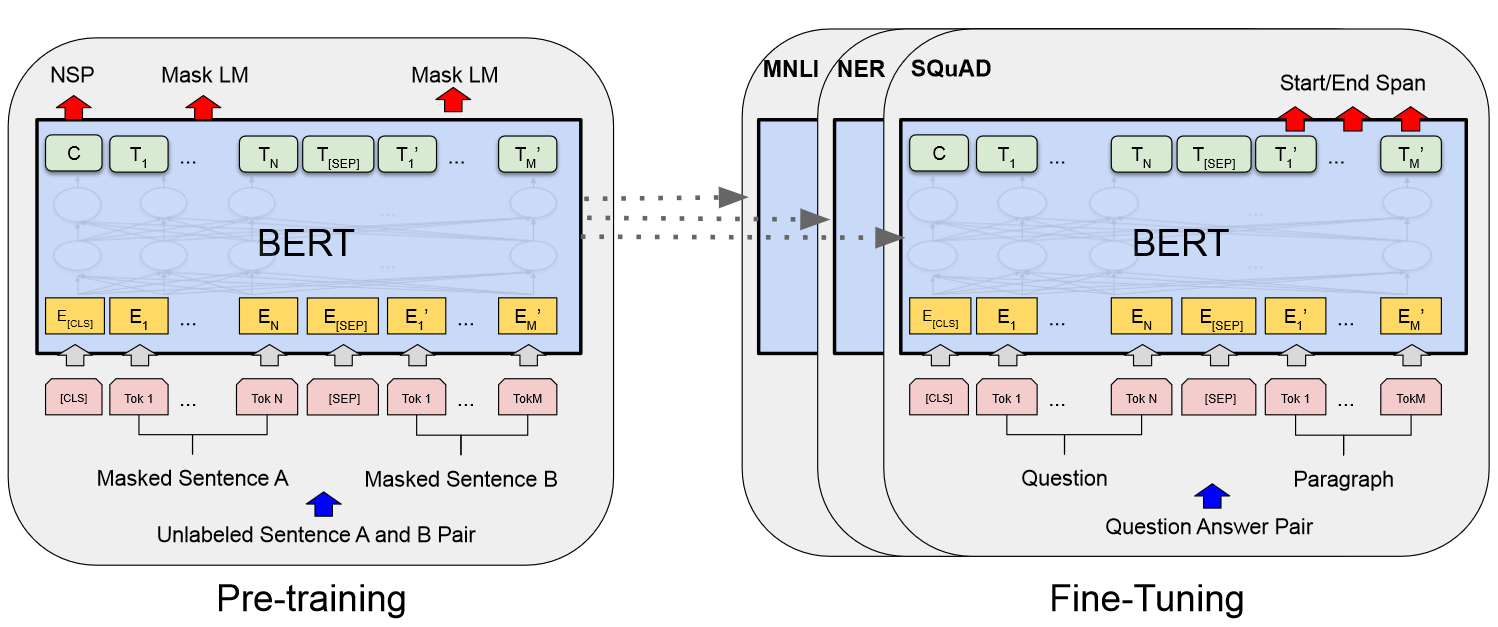
\includegraphics[scale=0.22]{./content/BERT_Architecture.png}
    \caption{Bidirectional Encoder Representations from Transformers (BERT) 
             schematic View \cite{devlin_bert_2019}.}
    \label{tab:bert}
\end{figure}

The Experiments are using BERT, Bidirectional Encoder Representations from Transformers (see Figure~\ref{tab:bert}) ~\cite{devlin_bert_2019} 
developed by Google is based on Transformer architecture introduced by Vaswani et al. \cite{vaswani_attention_2023}.
Unlike previous attempts, that process text in a unidirectional way (either left to right or right to 
left), BERT is designed to understand context bidirectionally as every Token is connected Pathways with every other. A masked language model (MLM) 
pre-training target is used, where tokens are randomly masked from the input to predict the original 
vocabulary IDs.
The model can be fine-tuned for specific downstream tasks, such as classification or translation. 
BERT is available in different sizes like BERT-Base and BERT-Large. There are various implementations 
such as RoBERTa~\cite{liu_roberta_2019}, ALBERT~\cite{lan_albert_2020}, BART~\cite{lewis_bart_2020}, 
DeBERTa~\cite{he_deberta_2021}, which improves BERT architecture differently.

We are using pre-trained BERT-Base Model from Huggingface~\cite{noauthor_hugging_2024-1} due to Limitations
of the Environment (see Chapter~\ref{ch:ev}) and supervised fine-tune it to SemEval.














\subsection{Sentence Embedding Architectures}\label{ch:seb}
\begin{figure}[!b]
    \vspace{-1cm}
    \centering
    %\resizebox{\textwidth}{!}{\begin{tikzpicture}
	\begin{pgfonlayer}{nodelayer}
		\node [style=rec] (0) at (0, 0) {Bert};
		\node [style=Textfeld] (1) at (0, 2) {Sentence};
		\node [style=rec] (2) at (0, -0.5) {For};
		\node [style=rec] (4) at (0, -1) {Sentence};
		\node [style=rec] (5) at (0, -1.5) {Classification};
		\node [style=Textfeld] (9) at (2.75, 2) {smt};
		\node [style=Textfeld] (10) at (4.25, 2) {sec};
		\node [style=Textfeld] (11) at (5.75, 2) {$p_1, p_2, ...$};
		\node [style=Textfeld] (12) at (7.25, 2) {$s_1, s_2, ...$};
		\node [style=Scale] (13) at (5, -2) {Cat(u, v, x, y)};
		\node [style=Softmax] (14) at (5, -2.75) {Classifier};
		\node [style=Linear] (15) at (2.75, 0) {BERT};
		\node [style=Linear] (16) at (4.25, 0) {BERT};
		\node [style=Linear] (17) at (5.75, 0) {BERT};
		\node [style=Linear] (18) at (7.25, 0) {BERT};
		\node [style=Textfeld] (19) at (0, -4) {0 or 1};
		\node [style=Textfeld] (20) at (5, -4) {0 or 1};
		\node [style=Textfeld] (21) at (11.25, 2) {smt};
		\node [style=Textfeld] (22) at (12.75, 2) {$s_1, s_2, ...$};
		\node [style=Textfeld] (23) at (12.75, 2.5) {$p_1, p_2, ...$};
		\node [style=Scale] (25) at (9.5, -2) {Cat(u, v)};
		\node [style=Softmax] (26) at (9.5, -2.75) {Classifier};
		\node [style=Linear] (27) at (11.25, 0) {BERT};
		\node [style=Linear] (28) at (12.75, 0) {BERT};
		\node [style=Textfeld] (31) at (9.5, -4) {0 or 1};
		\node [style=Textfeld] (32) at (12.75, 3) {sec};
		\node [style=Scale] (36) at (12, -2) {Cat(u, v, |u-v|)};
		\node [style=Softmax] (37) at (12, -2.75) {Classifier};
		\node [style=Textfeld] (40) at (12, -4) {0 or 1};
		\node [style=Scale] (45) at (14.5, -2) {CosSim(u, v)};
		\node [style=Softmax] (46) at (14.5, -2.75) {Map(-1, 1 -> 0, 1)};
		\node [style=Textfeld] (49) at (14.5, -4) {0 or 1};
		\node [style=none] (51) at (1.75, 3) {};
		\node [style=none] (52) at (1.75, -5.25) {};
		\node [style=none] (53) at (8.25, 3) {};
		\node [style=none] (54) at (8.25, -5.25) {};
		\node [style=Textfeld] (55) at (0, -5) {\textbf{v1/Baseline}};
		\node [style=Textfeld] (56) at (5, -5) {\textbf{v2}};
		\node [style=Textfeld] (57) at (9.5, -5) {\textbf{v3}};
		\node [style=Textfeld] (58) at (12, -5) {\textbf{v4}};
		\node [style=Textfeld] (59) at (14.5, -5) {\textbf{v5/v6}};
		\node [style=none] (60) at (-1.25, -4.5) {};
		\node [style=none] (61) at (16, -4.5) {};
	\end{pgfonlayer}
	\begin{pgfonlayer}{edgelayer}
		\draw [style=arrow] (1) to (0);
		\draw [style=arrow] (13) to (14);
		\draw [style=arrow] (9) to (15);
		\draw [style=arrow] (15) to (13);
		\draw [style=arrow] (16) to (13);
		\draw [style=arrow] (10) to (16);
		\draw [style=arrow] (11) to (17);
		\draw [style=arrow] (17) to (13);
		\draw [style=arrow] (12) to (18);
		\draw [style=arrow] (18) to (13);
		\draw [style=arrow] (5) to (19);
		\draw [style=arrow] (14) to (20);
		\draw [style=arrow] (25) to (26);
		\draw [style=arrow] (21) to (27);
		\draw [style=arrow] (27) to (25);
		\draw [style=arrow] (28) to (25);
		\draw [style=arrow] (22) to (28);
		\draw [style=arrow] (26) to (31);
		\draw [style=arrow] (36) to (37);
		\draw [style=arrow] (37) to (40);
		\draw [style=arrow] (45) to (46);
		\draw [style=arrow] (46) to (49);
		\draw (51.center) to (52.center);
		\draw [style=arrow] (27) to (36);
		\draw [style=arrow] (27) to (45);
		\draw [style=arrow] (28) to (36);
		\draw [style=arrow] (28) to (45);
		\draw (53.center) to (54.center);
		\draw (60.center) to (61.center);
	\end{pgfonlayer}
\end{tikzpicture}
}
    \resizebox{\textwidth}{!}{\begin{tikzpicture}
	\begin{pgfonlayer}{nodelayer}
		\node [style=rec] (0) at (0, 0) {Bert};
		\node [style=Textfeld] (1) at (0, 2) {Sentence};
		\node [style=rec] (2) at (0, -0.5) {For};
		\node [style=rec] (4) at (0, -1) {Sentence};
		\node [style=rec] (5) at (0, -1.5) {Classification};
		\node [style=Textfeld] (9) at (2.75, 2) {smt};
		\node [style=Textfeld] (10) at (4.25, 2) {sec};
		\node [style=Textfeld] (11) at (5.75, 2) {$p_1, p_2, ...$};
		\node [style=Textfeld] (12) at (7.25, 2) {$s_1, s_2, ...$};
		\node [style=Scale] (13) at (5, -2) {Cat(u, v, x, y)};
		\node [style=Softmax] (14) at (5, -2.75) {Classifier};
		\node [style=Linear] (15) at (2.75, 0) {BERT};
		\node [style=Linear] (16) at (4.25, 0) {BERT};
		\node [style=Linear] (17) at (5.75, 0) {BERT};
		\node [style=Linear] (18) at (7.25, 0) {BERT};
		\node [style=Textfeld] (19) at (0, -4) {0 or 1};
		\node [style=Textfeld] (20) at (5, -4) {0 or 1};
		\node [style=Textfeld] (21) at (11.25, 2) {smt};
		\node [style=Textfeld] (22) at (12.75, 2) {$s_1, s_2, ...$};
		\node [style=Textfeld] (23) at (12.75, 2.5) {$p_1, p_2, ...$};
		\node [style=Scale] (25) at (9.5, -2) {Cat(u, v)};
		\node [style=Softmax] (26) at (9.5, -2.75) {Classifier};
		\node [style=Linear] (27) at (11.25, 0) {BERT};
		\node [style=Linear] (28) at (12.75, 0) {BERT};
		\node [style=Textfeld] (31) at (9.5, -4) {0 or 1};
		\node [style=Textfeld] (32) at (12.75, 3) {sec};
		\node [style=Scale] (36) at (12, -2) {Cat(u, v, |u-v|)};
		\node [style=Softmax] (37) at (12, -2.75) {Classifier};
		\node [style=Textfeld] (40) at (12, -4) {0 or 1};
		\node [style=Scale] (45) at (14.5, -2) {CosSim(u, v)};
		\node [style=Softmax] (46) at (14.5, -2.75) {Map(-1, 1 -> 0, 1)};
		\node [style=Textfeld] (49) at (14.5, -4) {0 or 1};
		\node [style=none] (51) at (1.75, 3) {};
		\node [style=none] (52) at (1.75, -5.25) {};
		\node [style=none] (53) at (8.25, 3) {};
		\node [style=none] (54) at (8.25, -5.25) {};
		\node [style=Textfeld] (55) at (0, -5) {\textbf{v1/Baseline}};
		\node [style=Textfeld] (56) at (5, -5) {\textbf{v2}};
		\node [style=Textfeld] (57) at (9.5, -5) {\textbf{v3}};
		\node [style=Textfeld] (58) at (12, -5) {\textbf{v4}};
		\node [style=Textfeld] (59) at (14.5, -5) {\textbf{v5/v6}};
		\node [style=none] (60) at (-1.25, -4.5) {};
		\node [style=none] (61) at (16, -4.5) {};
	\end{pgfonlayer}
	\begin{pgfonlayer}{edgelayer}
		\draw [style=arrow] (1) to (0);
		\draw [style=arrow] (13) to (14);
		\draw [style=arrow] (9) to (15);
		\draw [style=arrow] (15) to (13);
		\draw [style=arrow] (16) to (13);
		\draw [style=arrow] (10) to (16);
		\draw [style=arrow] (11) to (17);
		\draw [style=arrow] (17) to (13);
		\draw [style=arrow] (12) to (18);
		\draw [style=arrow] (18) to (13);
		\draw [style=arrow] (5) to (19);
		\draw [style=arrow] (14) to (20);
		\draw [style=arrow] (25) to (26);
		\draw [style=arrow] (21) to (27);
		\draw [style=arrow] (27) to (25);
		\draw [style=arrow] (28) to (25);
		\draw [style=arrow] (22) to (28);
		\draw [style=arrow] (26) to (31);
		\draw [style=arrow] (36) to (37);
		\draw [style=arrow] (37) to (40);
		\draw [style=arrow] (45) to (46);
		\draw [style=arrow] (46) to (49);
		\draw (51.center) to (52.center);
		\draw [style=arrow] (27) to (36);
		\draw [style=arrow] (27) to (45);
		\draw [style=arrow] (28) to (36);
		\draw [style=arrow] (28) to (45);
		\draw (53.center) to (54.center);
		\draw (60.center) to (61.center);
	\end{pgfonlayer}
\end{tikzpicture}
}
    \caption{Sentence Embedding idea is based on BERT Model. Strategy v1 is the
             Baseline, handling everything in once and every token can contribute to each other, while
             Strategy v2 split the sentence in four parts, and fed separately to the same
             model. Strategy v3, v4, v5 and v6
             uses the same idea but Concatenating, using only premise and hypothesis and generating the output differently.}\label{fig:ver}
\end{figure}

Sentence-BERT (SBERT) \cite{reimers_sentence-bert_2019}, a modification of the BERT \cite{devlin_bert_2019} network, is a strategy designed for 
semantic similarity tasks, to generate meaningful embeddings. While BERT \cite{devlin_bert_2019} and RoBERTa \cite{liu_roberta_2019} excel in sentence-pair 
regression tasks, they suffer from computational overhead when dealing with large 
collections of sentences. SBERT addresses this issue by using 
siamese and triplet network structures to generate semantically meaningful 
sentence embeddings. Also, a key point is, especially with BERT, the two sentences are 
passing the Model individual, meaning that the Tokens of each sentence does not interfere
with each other. This allows for efficient similarity comparisons, 
clustering, and semantic search.
The authors demonstrate that SBERT significantly reduces the time required for 
finding the most similar pair in a collection of 10,000 sentences from 65 
hours with BERT to about 5 seconds.

We use this Principle and applied it to the SemEval Task (see Figure~\ref{fig:ver}). 
Therefore, we come up with five different ideas, where they use the Siamese-Architecture as Core, 
which is sharing the Models Parameters. Version-2 (v2) has four
parts of the defined Sentence (see Equation~\ref{eq:ds-sentence}) split at the $[SEP]$ Tokens.
Version-3 (v3), Version-4 (v4), Version-5 (v5) and Version-6 (v6) has the split on the first $[SEP]$ Token, to separate Statement from the Hypothesis.
Version-3 and Version-4 uses a simple Feed-Forward-Classifier after the Concatenation combined with CrossEntropyLoss.
Version-5 and Version-6 uses Cosine Similarity, with a Mapping ensuring Entailment being $1$ and
Contradiction being $-1$. Version-5 uses CosineEmbeddingLoss and Version-6 uses MSELoss to 
minimize, if entailed, and maximize, if contradiction, the spatial distances.


















\subsection{Adapter Tuning}\label{ch:adapter}

Adapter Tuning (see Figure~\ref{tab:adapt}) is a supervised method, where input, gold label are given and the models parameters are frozen, 
but adding new fully trainable bottleneck feed-forward networks 
on each intermediate layer. The objective is to reduce the size of trainable parameters, 
to gain higher throughput and keeping the pre-trained embeddings\cite{zheng_learn_2023} \cite{naveed_comprehensive_2023}. 
The ultimate goal of adaptation training is to enhance the model's scores on the downstream task, 
while still benefiting from the broad language understanding gained during the initial 
pre-training \cite{manjavacas_adapting_2022}. The effectiveness of adaptation-tuning depends on 
the similarity between the pre-training task and the target task due to fixed embeddings.

\begin{figure}[!b]
    \centering
    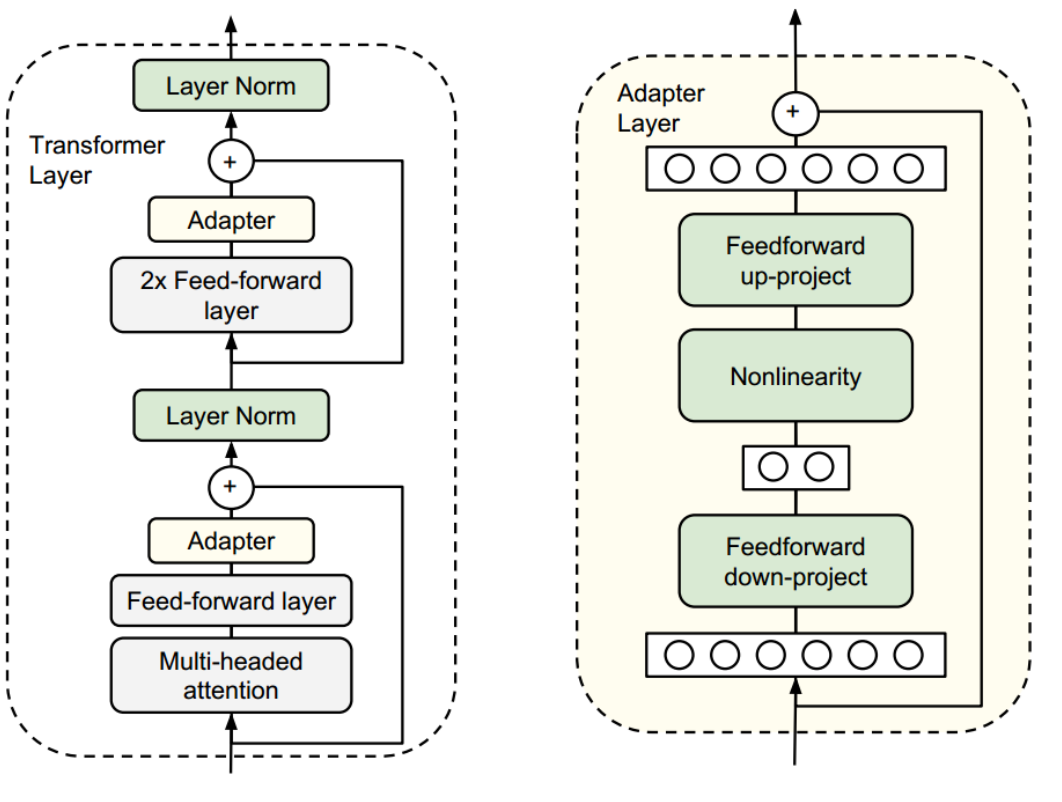
\includegraphics[scale=0.25]{./content/Adapter_Architecture.png}
    \caption{Basic Structure of Adapter built on top of a Models Architecture (left side), where only the Adapter Layers Parameters (right side) are trainable \cite{zheng_learn_2023}.
             In our Case we are using $768$ to $512$ DOWN-Projector, followed by GELU-Activation and
             $512$ to $768$ UP-Projector.}
    \label{tab:adapt}
\end{figure}


For our Experiments we are comparing supervised fine-tuned BERT, with the SemEval dataset against
a Adapter-BERT version, where the pre-trained BERT's Parameters are frozen. Secondly we are
taking the BERT Model from SimCSE~\cite{gao_simcse_2022-1}, which applied a Supervised
Contrastive Learning idea on SNLI Data, to minimize and maximize the spatial distances,
which effects the Output Representations of BERT and using the same principle with the Adapter on this Model.







\subsection{Loss Functions and Evaluation Metric}
We are using 3 commonly used Loss functions for our Training of the different
Architectures with $x$ being the Prediction and $y$ being the searched Class. For direct Classification, 
CrossEntropyLoss~\ref{eq:ce} is the commonly and most frequently used function. Secondly, as we see later,
combined with Cosine Simmilarity, we are using MSELoss~\ref{eq:mse} or CosineEmbeddingLoss~\ref{eq:ceb}
to maximize or minimize the distance between two representations. As Metric the SemEval Task uses F1 Score, which
is the harmonic mean between precision and recall defined in Equation~\ref{eq:f} \cite{noauthor_nli4ct_nodate}.



\begin{equation}\label{eq:ce}
   Loss_{CE} = -\sum_{i=1}^My_{o,i}\log(x_{o,i})
\end{equation}
\begin{equation}\label{eq:mse}
   Loss_{MSE} = \sum_{i=1}^{M}(x_i-y_i)^2
\end{equation}

\begin{equation}\label{eq:ceb}
    Loss_{CEB} = \begin{cases}
        1 - \cos(x_1, x_2),      &\text{if $y = +1$}\\
        \max(0, \cos(x_1, x_2)), &\text{if $y = -1$}
    \end{cases}
\end{equation}

\begin{equation}\label{eq:f}
    F_1 = 2 \frac{precision \cdot recall}{precision + recall} = \frac{2 TP}{2TP + FP + FN}
 \end{equation}


 



\subsection{Fusing different Datasets/Loaders}
\begin{figure}[b]
    \centering
    \resizebox{\textwidth}{!}{\begin{tikzpicture}
	\begin{pgfonlayer}{nodelayer}
		\node [style=base] (0) at (0, 0) {};
		\node [style=1x1 v1] (1) at (-7.5, 0) {};
		\node [style=1x1 v1] (4) at (-6.5, 0) {};
		\node [style=1x1 v1] (6) at (-5.5, 0) {};
		\node [style=1x1 v1] (7) at (-4.5, 0) {};
		\node [style=1x1 v3] (9) at (-3.5, 0) {};
		\node [style=1x1 v3] (10) at (-2.5, 0) {};
		\node [style=1x1 v3] (11) at (-1.5, 0) {};
		\node [style=1x1 v3] (12) at (-0.5, 0) {};
		\node [style=1x1 v4] (35) at (0.5, 0) {};
		\node [style=1x1 v4] (36) at (1.5, 0) {};
		\node [style=1x1 v4] (37) at (2.5, 0) {};
		\node [style=1x1 v4] (38) at (3.5, 0) {};
		\node [style=1x1 v2] (39) at (4.5, 0) {};
		\node [style=1x1 v2] (40) at (5.5, 0) {};
		\node [style=1x1 v2] (41) at (6.5, 0) {};
		\node [style=1x1 v2] (42) at (7.5, 0) {};
		\node [style=base] (43) at (19, 0) {};
		\node [style=1x1 v1] (44) at (11.5, 0) {};
		\node [style=1x1 v1] (45) at (12.5, 0) {};
		\node [style=1x1 v1] (46) at (13.5, 0) {};
		\node [style=1x1 v1] (47) at (14.5, 0) {};
		\node [style=1x1 v3] (48) at (15.5, 0) {};
		\node [style=1x1 v3] (49) at (16.5, 0) {};
		\node [style=1x1 v4] (52) at (17.5, 0) {};
		\node [style=1x1 v2] (56) at (19.5, 0) {};
		\node [style=1x1 v2] (57) at (24.5, 0) {};
		\node [style=1x1 v2] (58) at (25.5, 0) {};
		\node [style=1x1 v2] (59) at (26.5, 0) {};
		\node [style=base] (60) at (0, -3) {};
		\node [style=1x1 v1] (61) at (-7.5, -3) {};
		\node [style=1x1 v1] (62) at (-6.5, -3) {};
		\node [style=1x1 v1] (63) at (-5.5, -3) {};
		\node [style=1x1 v1] (64) at (-4.5, -3) {};
		\node [style=1x1 v3] (65) at (-3.5, -3) {};
		\node [style=1x1 v3] (66) at (-2.5, -3) {};
		\node [style=1x1 v3] (67) at (-1.5, -3) {};
		\node [style=1x1 v3] (68) at (-0.5, -3) {};
		\node [style=1x1 v4] (69) at (0.5, -3) {};
		\node [style=1x1 v4] (70) at (1.5, -3) {};
		\node [style=1x1 v4] (71) at (2.5, -3) {};
		\node [style=1x1 v4] (72) at (3.5, -3) {};
		\node [style=1x1 v2] (73) at (4.5, -3) {};
		\node [style=1x1 v2] (74) at (5.5, -3) {};
		\node [style=1x1 v2] (75) at (6.5, -3) {};
		\node [style=1x1 v2] (76) at (7.5, -3) {};
		\node [style=base] (77) at (0, -1.5) {};
		\node [style=1x1 v1] (78) at (-7.5, -1.5) {};
		\node [style=1x1 v1] (79) at (-6.5, -1.5) {};
		\node [style=1x1 v1] (80) at (-5.5, -1.5) {};
		\node [style=1x1 v1] (81) at (-4.5, -1.5) {};
		\node [style=1x1 v3] (82) at (-3.5, -1.5) {};
		\node [style=1x1 v3] (83) at (-2.5, -1.5) {};
		\node [style=1x1 v3] (84) at (-1.5, -1.5) {};
		\node [style=1x1 v3] (85) at (-0.5, -1.5) {};
		\node [style=1x1 v4] (86) at (0.5, -1.5) {};
		\node [style=1x1 v4] (87) at (1.5, -1.5) {};
		\node [style=1x1 v4] (88) at (2.5, -1.5) {};
		\node [style=1x1 v4] (89) at (3.5, -1.5) {};
		\node [style=1x1 v2] (90) at (4.5, -1.5) {};
		\node [style=1x1 v2] (91) at (5.5, -1.5) {};
		\node [style=1x1 v2] (92) at (6.5, -1.5) {};
		\node [style=1x1 v2] (93) at (7.5, -1.5) {};
		\node [style=base] (94) at (0, -4.5) {};
		\node [style=1x1 v1] (95) at (-7.5, -4.5) {};
		\node [style=1x1 v1] (96) at (-6.5, -4.5) {};
		\node [style=1x1 v1] (97) at (-5.5, -4.5) {};
		\node [style=1x1 v1] (98) at (-4.5, -4.5) {};
		\node [style=1x1 v3] (99) at (-3.5, -4.5) {};
		\node [style=1x1 v3] (100) at (-2.5, -4.5) {};
		\node [style=1x1 v3] (101) at (-1.5, -4.5) {};
		\node [style=1x1 v3] (102) at (-0.5, -4.5) {};
		\node [style=1x1 v4] (103) at (0.5, -4.5) {};
		\node [style=1x1 v4] (104) at (1.5, -4.5) {};
		\node [style=1x1 v4] (105) at (2.5, -4.5) {};
		\node [style=1x1 v4] (106) at (3.5, -4.5) {};
		\node [style=1x1 v2] (107) at (4.5, -4.5) {};
		\node [style=1x1 v2] (108) at (5.5, -4.5) {};
		\node [style=1x1 v2] (109) at (6.5, -4.5) {};
		\node [style=1x1 v2] (110) at (7.5, -4.5) {};
		\node [style=1x1 v1] (111) at (20.5, 0) {};
		\node [style=1x1 v1] (112) at (21.5, 0) {};
		\node [style=1x1 v3] (113) at (22.5, 0) {};
		\node [style=1x1 v2] (114) at (18.5, 0) {};
		\node [style=1x1 v4] (127) at (23.5, 0) {};
		\node [style=base] (128) at (19, -1.5) {};
		\node [style=1x1 v1] (129) at (11.5, -1.5) {};
		\node [style=1x1 v1] (130) at (12.5, -1.5) {};
		\node [style=1x1 v1] (131) at (13.5, -1.5) {};
		\node [style=1x1 v1] (132) at (14.5, -1.5) {};
		\node [style=1x1 v1] (140) at (20.5, -1.5) {};
		\node [style=1x1 v1] (141) at (21.5, -1.5) {};
		\node [style=1x1 v4] (144) at (19.5, -1.5) {};
		\node [style=1x1 v1] (145) at (15.5, -1.5) {};
		\node [style=1x1 v1] (146) at (16.5, -1.5) {};
		\node [style=1x1 v1] (147) at (17.5, -1.5) {};
		\node [style=1x1 v1] (148) at (18.5, -1.5) {};
		\node [style=1x1 v1] (149) at (22.5, -1.5) {};
		\node [style=1x1 v1] (150) at (23.5, -1.5) {};
		\node [style=1x1 v1] (151) at (24.5, -1.5) {};
		\node [style=1x1 v1] (152) at (25.5, -1.5) {};
		\node [style=1x1 v1] (153) at (26.5, -1.5) {};
		\node [style=base] (154) at (19, -3) {};
		\node [style=1x1 v1] (155) at (15.5, -3) {};
		\node [style=1x1 v1] (159) at (20.5, -3) {};
		\node [style=1x1 v1] (160) at (21.5, -3) {};
		\node [style=1x1 v4] (161) at (19.5, -3) {};
		\node [style=1x1 v1] (165) at (18.5, -3) {};
		\node [style=1x1 v1] (166) at (22.5, -3) {};
		\node [style=1x1 v1] (167) at (23.5, -3) {};
		\node [style=1x1 v1] (168) at (24.5, -3) {};
		\node [style=1x1 v1] (170) at (26.5, -3) {};
		\node [style=1x1 v4] (171) at (11.5, -3) {};
		\node [style=1x1 v4] (172) at (25.5, -3) {};
		\node [style=1x1 v4] (173) at (14.5, -3) {};
		\node [style=1x1 v3] (174) at (12.5, -3) {};
		\node [style=1x1 v2] (175) at (13.5, -3) {};
		\node [style=1x1 v2] (176) at (16.5, -3) {};
		\node [style=1x1 v2] (177) at (17.5, -3) {};
		\node [style=base] (178) at (19, -4.5) {};
		\node [style=1x1 v4] (182) at (19.5, -4.5) {};
		\node [style=1x1 v1] (183) at (18.5, -4.5) {};
		\node [style=1x1 v1] (185) at (23.5, -4.5) {};
		\node [style=1x1 v1] (186) at (24.5, -4.5) {};
		\node [style=1x1 v1] (187) at (26.5, -4.5) {};
		\node [style=1x1 v4] (188) at (12.5, -4.5) {};
		\node [style=1x1 v4] (189) at (25.5, -4.5) {};
		\node [style=1x1 v3] (191) at (11.5, -4.5) {};
		\node [style=1x1 v2] (192) at (13.5, -4.5) {};
		\node [style=1x1 v2] (193) at (16.5, -4.5) {};
		\node [style=1x1 v2] (194) at (17.5, -4.5) {};
		\node [style=1x1 v2] (195) at (14.5, -4.5) {};
		\node [style=1x1 v2] (196) at (15.5, -4.5) {};
		\node [style=1x1 v2] (197) at (20.5, -4.5) {};
		\node [style=1x1 v2] (198) at (21.5, -4.5) {};
		\node [style=1x1 v3] (199) at (22.5, -4.5) {};
		\node [style=Textfeld] (200) at (19, 1.25) {Combined Dataset};
		\node [style=Textfeld] (201) at (0, 1.25) {Combined Loader};
		\node [style=Textfeld] (202) at (9.5, 1.25) {Batch};
		\node [style=Textfeld] (203) at (9.5, 0) {1};
		\node [style=Textfeld] (204) at (9.5, -1.5) {2};
		\node [style=Textfeld] (205) at (9.5, -3) {...};
		\node [style=Textfeld] (206) at (9.5, -4.5) {n};
	\end{pgfonlayer}
\end{tikzpicture}
}
    \caption{Combined Dataset and Combined Loader Strategy where 4 different Datasets are getting mixed together.
             On the Loader-Level for a Batch size of 16, every Dataset is present equally and on the
             Dataset-Level, they are concatenated and the mixed.}\label{fig:test}
\end{figure}


Normally a Pre-Trained Model is used which is then fine-tuned on the Specific Dataset. The same can be applied to
Text Classification. Therefore, the Model is performing only on SemEval very good, while mismatching on generalization
on other Text Classification Tasks. To Compensate, two strategies (see Figure~\ref{fig:test}) are applied to solve this.
CombinedLoaders is a strategy, where each Dataset, on which the Model should perform, can contribute equally with
the same amount of Datapoints. Another strategy involves the concatenation of all these Datasets to one and then being
mixed on the Training. For our Example (see Chapter~\ref{ch:ds} and Figure~\ref{tab:histo}) we are using SNLI \cite{noauthor_snli_2023}
which has short sentences for entailment check, HEALTHVER \cite{noauthor_dwaddenhealthver_entailment_nodate} a Dataset on the medical domain and
SCIFACT \cite{noauthor_allenaiscifact_entailment_nodate} on the scientific domain, to check the entailment of claim, 
paper title and abstract. The Evaluation of the Strategies is only applied to SemEval Task Development
Dataset not on the chosen ones for expanding. Also, the expected outcome should be lower than the
specialized Model on SemEval as it has to generalize the different domains.


\begin{figure}[t]
    \hspace*{-1.75cm}
    \centering
    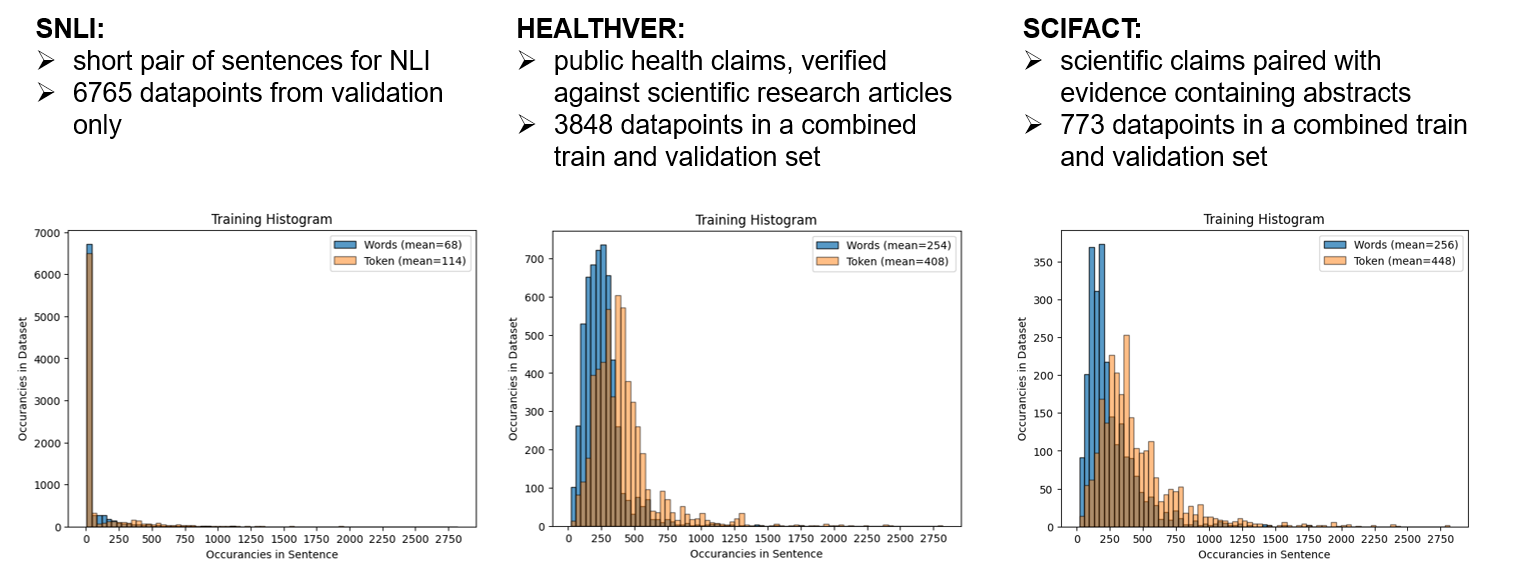
\includegraphics[width=1.3\textwidth]{./content/Histogram_Dataset.png}
    \caption{Histogram of how different Datasets combined with SemEval changes the
             Occurrences in the Bins. HEALTHVER and SCIFACT shows a slight
             shift on the x-Axis towards right, indicating that the length
             of the sentences is higher. On the other side SNLI, is dominating, 
             because the sentence structure is rather small. }
    \label{tab:histo}
\end{figure}























\newpage
\section{Experiments}\label{sec:experiments}

\subsection{Environmental Setup}\label{ch:ev}
For our Experiments we are bounded by the Environments given from Kaggle \cite{noauthor_kaggle_nodate} and Colab \cite{noauthor_google_nodate}, 
which makes quite complex to find the optimal hyperparameter. Also, there is no possibility to Cache or Precalculate all the Datapoints of
Training and Validation without running in to RAM issues. We decided to shift the bottlenecks either in parallel loading the
Data and/or running in exceeding GPU RAM due to the amount of parameters.

\vspace{0.3cm}

\begin{minipage}{0.5\textwidth}
    Colab's Environment:
    \begin{itemize}
        \item CPU: Intel(R) Xeon(R) @ 2.00GHz
        \item Number of available Cores: 2
        \item System Ram: 12 GB
        \item GPU: Nvidia Tesla T4
        \item GPU Ram: 15 GB
        \item Time limit: 3-4 Hours a Day/Session
    \end{itemize}
\end{minipage}
\begin{minipage}{0.5\textwidth}
    Kaggle's Environment:
    \begin{itemize}
        \item CPU: Intel(R) Xeon(R) @ 2.00GHz
        \item Number of available Cores: 4
        \item System Ram: 32 GB
        \item GPU: Nvidia Tesla P100
        \item GPU Ram: 16 GB
        \item Time limit: 30 Hour a Week with 9h each Session
    \end{itemize}
\end{minipage}

\vspace{0.3cm}

The general handling of the loops is based on Pytorch \cite{noauthor_pytorch_nodate}, Lightning AI \cite{noauthor_lightning_nodate}
implementation and for loading the pre-trained BERT Model we are using Huggingface (transformer library) \cite{noauthor_hugging_2023}.
Therefore, we can focus the Experiments on implementing strategies to enhance BERT's overall performance tested on four different Seeds.











\subsection{Learning Rate}

In the evaluation of the Baseline BertModelForSentenceClassification, different Learning-Rate 
were tested, accompanied by variations in token size and the implementation of mixed precision.
The tested Range of Learning-Rate (see Table~\ref{tab:my-lr}) going from $3e-6$ to $7e-6$. All above or
below leading that the Model does not learn well or resulting in a rectangle graph, indicating
that the gradients are too high or low. The best Learning Rate, based on the Seeds is $6e-6$ with
$0.640 \pm 0.021$.

However, it was observed that altering the token size and introducing mixed precision led to 
the destruction of tensors within the model leading to re pre-train it whitin the Environment
this is impossible. 
This suggests potential challenges and limitations associated with modifying these parameters, 
emphasizing the need for careful consideration and experimentation when adjusting 
learning rates and employing mixed precision in the context of sentence classification 
tasks using the BERT model.

\begin{table}[h]
    \centering
    \caption{F1 Values of the Baseline BertModelForSentenceClassification of the Last (50th) Epoch
             for different Learning-Rates.}
    \label{tab:my-lr}
    \begin{tabular}{|c||cccc|c|}
    \hline
    \multicolumn{1}{|l||}{\multirow{2}{*}{Learning Rate}} & \multicolumn{4}{c|}{Seed}                                                                    & \multicolumn{1}{c|}{\multirow{2}{*}{mean $\pm$ std}} \\ \cline{2-5}
    \multicolumn{1}{|l||}{}                               & \multicolumn{1}{c|}{0}     & \multicolumn{1}{c|}{42}    & \multicolumn{1}{c|}{1998}  & 1M    & \multicolumn{1}{c|}{}                                \\ \hline\hline
    3e-6                                                 & \multicolumn{1}{c|}{0.637} & \multicolumn{1}{c|}{0.554} & \multicolumn{1}{c|}{0.623} & 0.652 & 0.614 $\pm$ 0.034                           \\ \hline
    4e-6                                                 & \multicolumn{1}{c|}{0.589} & \multicolumn{1}{c|}{0.614} & \multicolumn{1}{c|}{0.649} & 0.615 & 0.616 $\pm$ 0.019                                    \\ \hline
    5e-6                                                 & \multicolumn{1}{c|}{0.636} & \multicolumn{1}{c|}{0.640} & \multicolumn{1}{c|}{0.638} & 0.657 & 0.630 $\pm$ 0.026                                    \\ \hline
    6e-6                                                 & \multicolumn{1}{c|}{0.661} & \multicolumn{1}{c|}{0.654} & \multicolumn{1}{c|}{0.602} & 0.647 & \textbf{0.640 $\pm$ 0.021}                                    \\ \hline
    7e-6                                                 & \multicolumn{1}{c|}{0.644} & \multicolumn{1}{c|}{0.563} & \multicolumn{1}{c|}{0.657} & 0.655 & 0.621 $\pm$ 0.040                                    \\ \hline
    \end{tabular}
\end{table}
\vspace{-0.5cm}











\subsection{Permutation}
\begin{equation}\label{eq:permutate}
    \resizebox{0.91\hsize}{!}{%
     $Sentence = [CLS] \; \textcolor{red}{stm}\;
                 [SEP] \; \textcolor{green}{sec}\;
                 [SEP] \; \textcolor{blue}{\pi(p_1), \pi(p_2), ... }\;
                 [SEP] \; \textcolor{blue}{\pi(s_1), \pi(s_2), ... }\;
                 [SEP]$      
    }
\end{equation}

As described above changing Token size does lead to destroying the embeddings due to newly
initializing and the fact that the maximum token size is 512, we come up with the idea
of permuting the Primary and Secondary Trials (see Equation~\ref{eq:permutate}), which can be seen as list of items.
The Target to analyze is if the order of the elements is relevant for deciding the Prediction, 
wich should not be relevant due to BERT's Architecture, and
if information after the cutpoint has interesting and relevant facts, which influences
the decision making process. With no permutation the 
Sentence is only 512 tokens long with the first-come-first-serve principle. Permutation on
indicates that the order is not significant.

\begin{table}[!t]
    \centering
    \caption{F1 Values of the Permutation trial on the Baseline Model from the last (50th) Epoch}
    \label{tab:my-permutation}
    \begin{tabular}{|c|c||cccc|c|}
    \hline
    \multirow{2}{*}{Learning Rate} & \multirow{2}{*}{Permutation} & \multicolumn{4}{c|}{Seed}                                                                    & \multirow{2}{*}{mean $\pm$ std} \\ \cline{3-6}
                                   &                              & \multicolumn{1}{c|}{0}     & \multicolumn{1}{c|}{42}    & \multicolumn{1}{c|}{1998}  & 1M    &                                 \\ \hline \hline
    \multirow{2}{*}{5e-6}          & No                           & \multicolumn{1}{c|}{0.636} & \multicolumn{1}{c|}{0.640} & \multicolumn{1}{c|}{0.638} & 0.657 & 0.630 $\pm$ 0.026               \\ \cline{2-7} 
                                   & Yes                          & \multicolumn{1}{c|}{0.633} & \multicolumn{1}{c|}{0.652} & \multicolumn{1}{c|}{0.620} & 0.643 & \textbf{0.643 $\pm$ 0.016}      \\ \hline
    \end{tabular}
\end{table}

The Results (see Table~\ref{tab:my-permutation}) showed that there can be a slight Performance boost and the standard deviation is lower
indicating that the fluctuation of different seeds in not that harsh. But, the Runtime cost of permuting the
sentences every Batch is for the later Experiments too much. Therefore, we skip it to stay cost-efficient.














\subsection{Dataset Expansion}\label{ch:ds}

\begin{table}[!b]
    \centering
    \caption{F1 Values of the Dataset Expansion Test of Last (50th) Epoch for the different Startegies and Datasets, which are expanding SemEval. The Values are the SemEval only Validation.}
    \label{tab:my-dsexp}
    \resizebox{\textwidth}{!}{%
    \begin{tabular}{|c||cc|cccc|c|}
    \hline
    \multirow{2}{*}{Dataset + SemEval} & \multicolumn{2}{c|}{Strategy}        & \multicolumn{4}{c|}{Seed}                                                                    & \multirow{2}{*}{mean $\pm$ std} \\ \cline{2-7}
                                       & \multicolumn{1}{c|}{CombDL} & CombDS & \multicolumn{1}{c|}{0}     & \multicolumn{1}{c|}{42}    & \multicolumn{1}{c|}{1998}  & 1M    &                                 \\ \hline\hline
    Baseline                           & \multicolumn{1}{c|}{}       &        & \multicolumn{1}{c|}{0.636} & \multicolumn{1}{c|}{0.640} & \multicolumn{1}{c|}{0.638} & 0.657 & 0.630 $\pm$ 0.026               \\ \hline\hline
    
    \multirow{2}{*}{SNLI}              & \multicolumn{1}{c|}{\chm}   &        & \multicolumn{1}{c|}{0.597} & \multicolumn{1}{c|}{0.613} & \multicolumn{1}{c|}{0.685} & 0.573 & 0.617 $\pm$ 0.042               \\ \cline{2-8} 
                                       & \multicolumn{1}{c|}{}       & \chm   & \multicolumn{1}{c|}{0.619} & \multicolumn{1}{c|}{0.669} & \multicolumn{1}{c|}{0.648} & 0.634 & 0.643 $\pm$ 0.019               \\ \hline
    
    \multirow{2}{*}{HEALTHVER}         & \multicolumn{1}{c|}{\chm}   &        & \multicolumn{1}{c|}{0.634} & \multicolumn{1}{c|}{0.614} & \multicolumn{1}{c|}{0.622} & 0.610 & 0.620 $\pm$ 0.009               \\ \cline{2-8} 
                                       & \multicolumn{1}{c|}{}       & \chm   & \multicolumn{1}{c|}{0.637} & \multicolumn{1}{c|}{0.661} & \multicolumn{1}{c|}{0.613} & 0.631 & 0.635 $\pm$ 0.017               \\ \hline
    
    \multirow{2}{*}{SCIFACT}           & \multicolumn{1}{c|}{\chm}   &        & \multicolumn{1}{c|}{0.586} & \multicolumn{1}{c|}{0.547} & \multicolumn{1}{c|}{0.603} & 0.561 & 0.574 $\pm$ 0.022               \\ \cline{2-8} 
                                       & \multicolumn{1}{c|}{}       & \chm   & \multicolumn{1}{c|}{0.687} & \multicolumn{1}{c|}{0.619} & \multicolumn{1}{c|}{0.664} & 0.645 & \textbf{0.654 $\pm$ 0.025}      \\ \hline\hline

    
    \multirow{2}{*}{SCIFACT,HEALTHVER} & \multicolumn{1}{c|}{\chm}   &        & \multicolumn{1}{c|}{0.580} & \multicolumn{1}{c|}{0.564} & \multicolumn{1}{c|}{0.551} & 0.570 & 0.566 $\pm$ 0.010               \\ \cline{2-8} 
                                       & \multicolumn{1}{c|}{}       & \chm   & \multicolumn{1}{c|}{0.664} & \multicolumn{1}{c|}{0.637} & \multicolumn{1}{c|}{0.657} & 0.649 & \textbf{0.652 $\pm$ 0.010}     \\ \hline
    
    \multirow{2}{*}{SCIFACT,SNLI}      & \multicolumn{1}{c|}{\chm}   &        & \multicolumn{1}{c|}{0.645} & \multicolumn{1}{c|}{0.607} & \multicolumn{1}{c|}{0.545} & 0.567 & 0.591 $\pm$ 0.039               \\ \cline{2-8} 
                                       & \multicolumn{1}{c|}{}       & \chm   & \multicolumn{1}{c|}{0.658} & \multicolumn{1}{c|}{0.574} & \multicolumn{1}{c|}{0.624} & 0.644 & 0.625 $\pm$ 0.032               \\ \hline
    
    \multirow{2}{*}{HEALTHVER,SNLI}    & \multicolumn{1}{c|}{\chm}   &        & \multicolumn{1}{c|}{0.615} & \multicolumn{1}{c|}{0.537} & \multicolumn{1}{c|}{0.615} & 0.658 & 0.606 $\pm$ 0.044               \\ \cline{2-8} 
                                       & \multicolumn{1}{c|}{}       & \chm   & \multicolumn{1}{c|}{0.667} & \multicolumn{1}{c|}{0.611} & \multicolumn{1}{c|}{0.664} & 0.602 & 0.636 $\pm$ 0.030               \\ \hline
    \end{tabular}%
    }
\end{table}

We have tested the two Dataset Expansion Strategies CombinedLoader (CombDL) and CombinedDataset (CombDS)
on two phases with the expasion Datasets SNLI, HEALTHVER and SCIFACT. The first Stage 
is combining one Dataset with SemEval Training and testing the performance only on SemEval
Validation. The second Stage including two datasets from the list and doing the same
Training and Validation as before. 


The Results (see Table~\ref{tab:my-dsexp}) showed that the CombinedLoader Strategy is worse than the Baseline, 
which indicates that the model has generalization issues if the dataset is present
with the same amount of Datapoints. Also, CombinedDataset Strategy is almost every
time better than the Baseline Model, with around 2\% Points gain of F1 Value, showing
that a generalized Model, handling multiple Text Entailment subtasks on different domain 
is possible. Secondly it is visible that SCIFACT in combination with SemEval has the highest
performance gain, which is the result of being tokenized around the same length of SemEval, therefore
the Model has to abstract more the general meaning of the sentences and the Dataset is not dominant,
meaning that the size is equally powerful.














\subsection{Sentence Embedding Architectures}

As Results (see Table~\ref{tab:my-seb}) of the different Architectures (defined in Chapter~\ref{ch:seb})
most of them are equally powerful than the Baseline. Version-3 is 1\% Point less than Version-4, which 
is expected due to we are giving more information to the Feed-Forward-Layer (FNN). Version-2 is better than
the Baseline but 4 times expensive in the backward calculations, which makes the performance boost neglectable.
Version-6, which is the Siamese-Network combined with Cosine Similarity of the two embeddings of the sentences
and MSELoss as Loss function, has a gain of 3.4\% F1-Value score, showing that Sentence Embedding can
help to improve the Metric-Scores on the Text Entailment Task.


\begin{table}[h]
    \centering
    \caption{F1 Values of the different Architecture from the Last (50th) Epoch, indicating that Sentence Embedding
             can boost the overall Performance.}
    \label{tab:my-seb}
    \begin{tabular}{|c|c||cccc|c|}
    \hline
    \multirow{2}{*}{Model} & \multirow{2}{*}{Desciption}                                                                       & \multicolumn{4}{c|}{Seed}                                                                    & \multirow{2}{*}{mean $\pm$ std} \\ \cline{3-6}
                           &                                                                                                   & \multicolumn{1}{c|}{0}     & \multicolumn{1}{c|}{42}    & \multicolumn{1}{c|}{1998}  & 1M    &                                 \\ \hline\hline
    Baseline               & \begin{tabular}[c]{@{}c@{}}BertModelForSequenceClassification\\ and CrossEntropyLoss\end{tabular} & \multicolumn{1}{c|}{0.636} & \multicolumn{1}{c|}{0.640} & \multicolumn{1}{c|}{0.638} & 0.657 & 0.630 $\pm$ 0.026               \\ \hline
    v2                     & \begin{tabular}[c]{@{}c@{}}(u, v, x, y) as input to FFN\\ and CrossEntropyLoss\end{tabular}       & \multicolumn{1}{c|}{0.652} & \multicolumn{1}{c|}{0.619} & \multicolumn{1}{c|}{0.604} & 0.664 & 0.635 $\pm$ 0.024               \\ \hline
    v3                     & \begin{tabular}[c]{@{}c@{}}(u, v) as input to FNN\\ and CrossEntropyLoss\end{tabular}             & \multicolumn{1}{c|}{0.708} & \multicolumn{1}{c|}{0.583} & \multicolumn{1}{c|}{0.573} & 0.611 & 0.619 $\pm$ 0.054               \\ \hline
    v4                     & \begin{tabular}[c]{@{}c@{}}(u, v, |u-v|) as input to FNN\\ and CrossEntropyLoss\end{tabular}      & \multicolumn{1}{c|}{0.638} & \multicolumn{1}{c|}{0.631} & \multicolumn{1}{c|}{0.618} & 0.640 & 0.632 $\pm$ 0.009               \\ \hline
    v5                     & \begin{tabular}[c]{@{}c@{}}CosSim(u, v)\\ and CosineEmbeddingLoss\end{tabular}                    & \multicolumn{1}{c|}{0.614} & \multicolumn{1}{c|}{0.603} & \multicolumn{1}{c|}{0.637} & 0.664 & 0.630 $\pm$ 0.023               \\ \hline
    v6                     & \begin{tabular}[c]{@{}c@{}}CosSim(u, v)\\ and MSELoss\end{tabular}                                & \multicolumn{1}{c|}{0.667} & \multicolumn{1}{c|}{0.675} & \multicolumn{1}{c|}{0.667} & 0.646 & \textbf{0.664 $\pm$ 0.011}               \\ \hline
    \end{tabular}
\end{table}











\newpage
\subsection{Adapter}

As said in Chapter~\ref{ch:adapter}, we are testing this Principle on SimCSE objective trained 
BERT Model and on general pre-trained BERT overridden the BertModelForSentenceClassification Class. Firstly the Adapter version of the general 
pre-trained BERT is around 2\% Points worse, which indicates that the remaining
trainable Parameters are not enough to get a meaningful representation for the Classification-Layer (see Table~\ref{tab:my-adapt}).
On the opposite side, taking the supervised fine-tuned SimCSE Model, which is trained on SNLI data, 
also a Text Entailment Task, shows a Performance boos from 1.5-2\% in F1 Score. Therefore, 
is important that the task correlate to each other, so the normal Layer of the BERT 
already have a good representation saved in the Tensor and the Adapter Layer only has to align these.


\begin{table}[!t]
    \centering
    \caption{F1 Values of the Adapter Trial from the Last (50th) Epoch for the general BERT Model and
             the supervise SimCSE objective trained BERT}
    \label{tab:my-adapt}
    \begin{tabular}{|l||cccc|c|}
    \hline
    \multicolumn{1}{|c||}{\multirow{2}{*}{Model}} & \multicolumn{4}{c|}{Seed}                                                                    & \multirow{2}{*}{mean $\pm$ std} \\ \cline{2-5}
    \multicolumn{1}{|c||}{}                       & \multicolumn{1}{c|}{0}     & \multicolumn{1}{c|}{42}    & \multicolumn{1}{c|}{1998}  & 1M    &                                 \\ \hline\hline
    Baseline BERT                                 & \multicolumn{1}{c|}{0.636} & \multicolumn{1}{c|}{0.640} & \multicolumn{1}{c|}{0.638} & 0.657 & 0.630 $\pm$ 0.026               \\ \hline
    Adapter BERT                                  & \multicolumn{1}{c|}{0.619} & \multicolumn{1}{c|}{0.587} & \multicolumn{1}{c|}{0.602} & 0.626 & 0.608 $\pm$ 0.015               \\ \hline
    Baseline SimCSE                               & \multicolumn{1}{c|}{0.598} & \multicolumn{1}{c|}{0.667} & \multicolumn{1}{c|}{0.696} & 0.640 & \textbf{0.650 $\pm$ 0.036}               \\ \hline
    Adapter SimCSE                                & \multicolumn{1}{c|}{0.643} & \multicolumn{1}{c|}{0.673} & \multicolumn{1}{c|}{0.615} & 0.654 & 0.646 $\pm$ 0.021      \\ \hline
    \end{tabular}
\end{table}


\newpage
\section{Conclution}

In conclusion, this paper presents a thorough investigation into text entailment classification, 
focusing on Clinical Trial Reports (CTR) annotation. Through careful dataset curation and 
experimentation using the SemEval task 2 dataset, the study explores various approaches, 
including BERT-based models and adapter tuning. Despite challenges in environmental setup, 
the findings highlight the importance of learning rate optimization, dataset expansion 
strategies, and sentence embedding architectures in influencing model performance. 
The paper contributes valuable insights to natural language processing research, 
particularly in clinical text analysis, and sets the stage for further exploration 
in related domains.
%\newpage
\endgroup

%
% ---- Bibliography ----
%
% BibTeX users should specify bibliography style 'splncs04'.
% References will then be sorted and formatted in the correct style.
%
\bibliographystyle{splncs04}
\bibliography{PrakNLP} %Filename

\end{document}
